\section{Aeropêndulo}
Os sistemas mecânicos têm como uma de suas característica os graus liberdade, o Aeropêndulo tem um grau de liberdade, sendo o ângulo $\theta$, assim o sistema tem apenas uma variável a ser controlada a partir do empuxo gerado pelas hélices, que por sua vez depende da velocidade angular do eixo do motor CC Série acoplado ao braço do Aeropêndulo. dessa forma, podemos analisar o sistema a partir da entrada e da saída, sendo a entrada a tensão no motor e a saída o ângulo $\theta$ do braço do Aeropêndulo.

\begin{figure}[!h]
	\centering
	\caption{Diagrama esquemático do Aeropêndulo.}
	\efbox{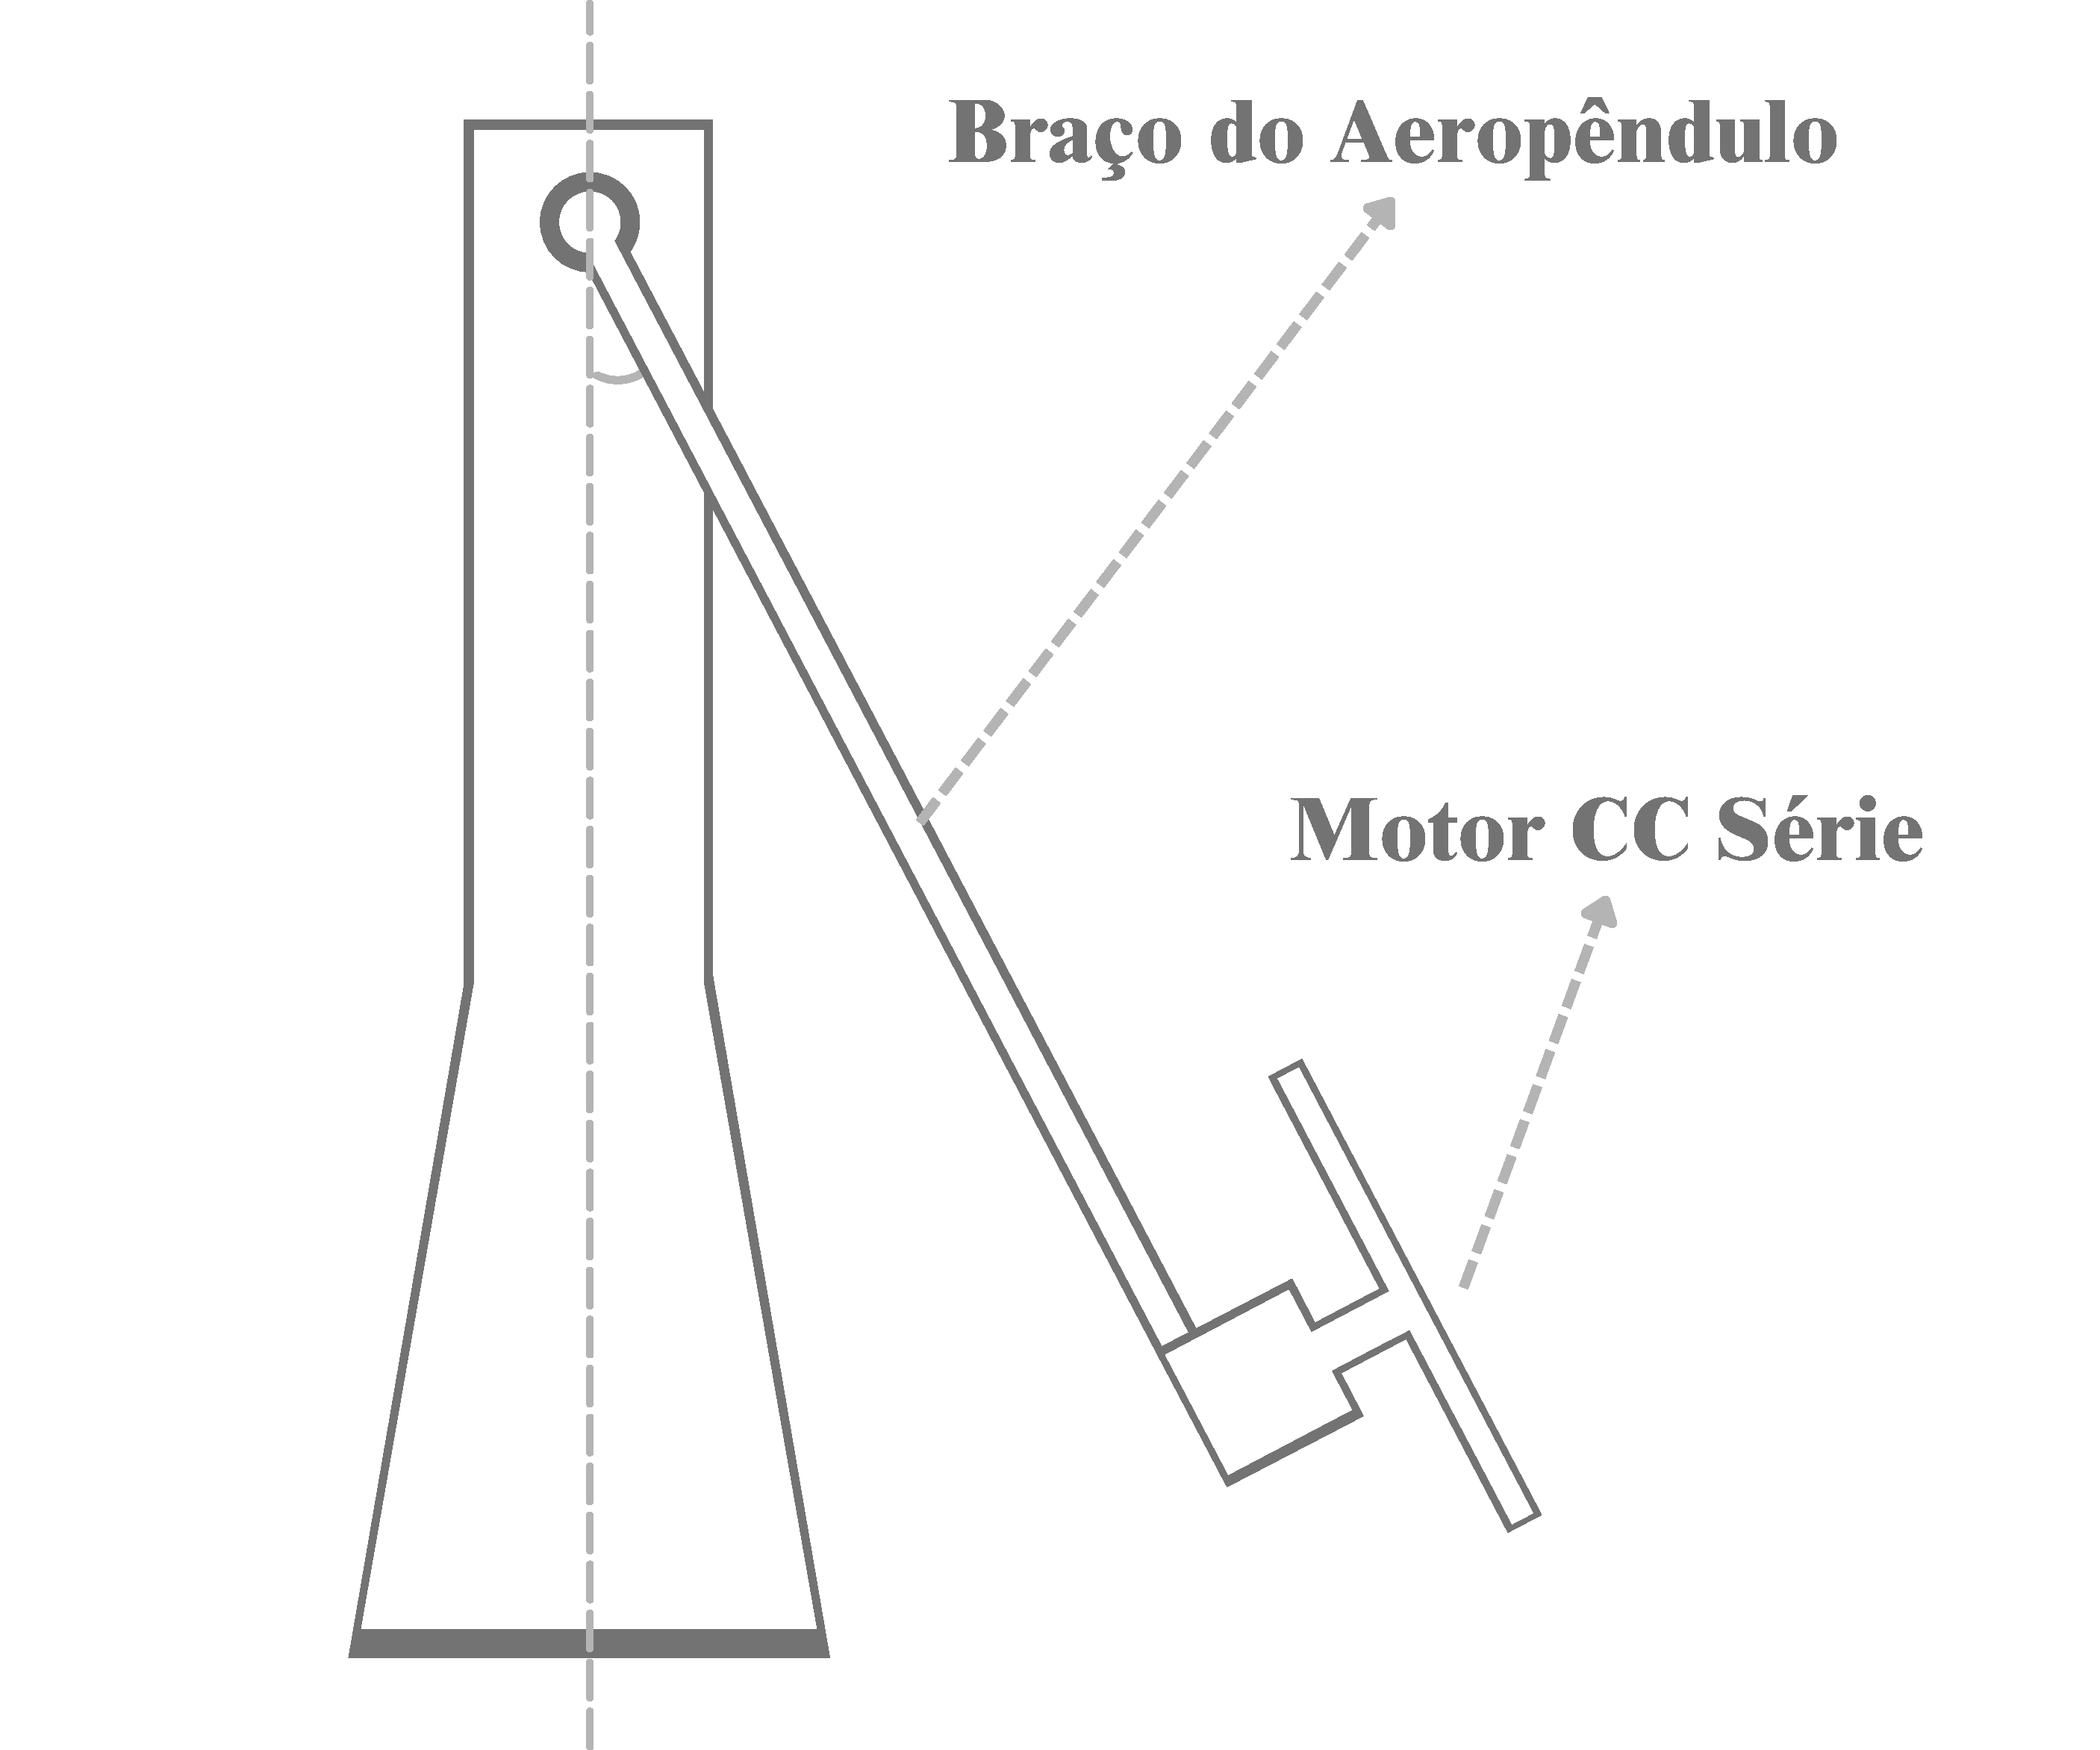
\includegraphics[width=0.55\textwidth]{Capitulos/2_aeropendulo/4_figuras/diagrama_aeropendulo_01.pdf}}
	\caption*{Fonte: elaborado pelo autor (2023).}
        \label{fig4:image_04}
\end{figure}




\section{ Fundamentação Teórica}
\label{fundamentacao_teorica}

O processo que envolve modelagem de sistemas físicos em termos de equações matemáticas é uma das partes mais importante no estudo de sistemas de controle. Segundo \citeonline[p.~11]{ogata5ed}, O modelo matemático de um sistema dinâmico é definido como um conjunto de equações que representa a dinâmica do sistema com precisão ou, pelo menos, razoavelmente bem.

A construção de modelos matemáticos adequados é fundamental na análise de sistemas de controle, pois a dinâmica de diversos sistemas, como mecânicos, elétricos, térmicos, econômicos, biológicos, entre outros, pode ser expressa por meio de equações diferenciais. Tais equações são derivadas das leis físicas que governam cada sistema específico, como as leis de Newton para sistemas mecânicos e as leis de Kirchhoff para sistemas elétricos. Esta abordagem ressalta a importância crucial de compreender as bases matemáticas subjacentes para uma análise abrangente dos sistemas de controle, conforme destacado por \citeonline[p.~11]{ogata5ed}.
